\documentclass[12pt, oneside]{article}
\usepackage{a4wide}
\usepackage{oldgerm}
\usepackage{amsmath}
\usepackage{amssymb}
\usepackage{amstext}
\usepackage{graphicx}
\setlength{\textheight}{8.875in} \setlength{\textwidth}{6.875in}
\setlength{\columnsep}{0.3125in} \setlength{\topmargin}{0in}
\setlength{\headheight}{0in} \setlength{\headsep}{0in}
\setlength{\parindent}{1pc} \setlength{\oddsidemargin}{-.304in}
\setlength{\evensidemargin}{-.304in}



\begin{document}
\setlength{\textheight}{8.5in}
\centering {\bf MTL 390 (Statistical Methods) }\\


\centering{\bf Minor Examination Assignment 1 Report}



\vskip 0.5cm

\noindent Name: Hetvi Jethwani ~~~~~~~~~~~~~~~~~~~ Entry Number: 2018MT10754 ~~~~~~~~~~~~~~



\vskip 0.5cm



\begin{enumerate}

\item Descriptive Statistics
\begin{enumerate}
    \item Jane went on the street and asked $n$ random people how many books they'd read in the past week for an assignment, she had stored all this data in a Google Sheet and later calculated the mean, coefficient of variation, kurtosis, and skew of the data as $\mu, \frac{s}{\mu},\gamma,\eta$ respectively. But then she got logged out of her Google account, and the only thing she has saved about the data is that the responses were in the range of $0-4,$ and the 4 descriptive values she calculated earlier. She won't be able to access her account for the next 24h but urgently has to turn in this assignment. Can we regain the original frequency table from the given variables? What's the best way to visualize this?
    \item While doing a literature review for similar studies, she sees the following box plot. Help her understand what the shape of each box plot tells us about the underlying distribution. Given that these plots are about the month-wise sales of paperbacks offline, sales of paperbacks online, and sales of ebooks in 2020 for India, match the distribution to the numbered box plot and justify your choice. 
    \begin{figure}[!ht]
        \centering
        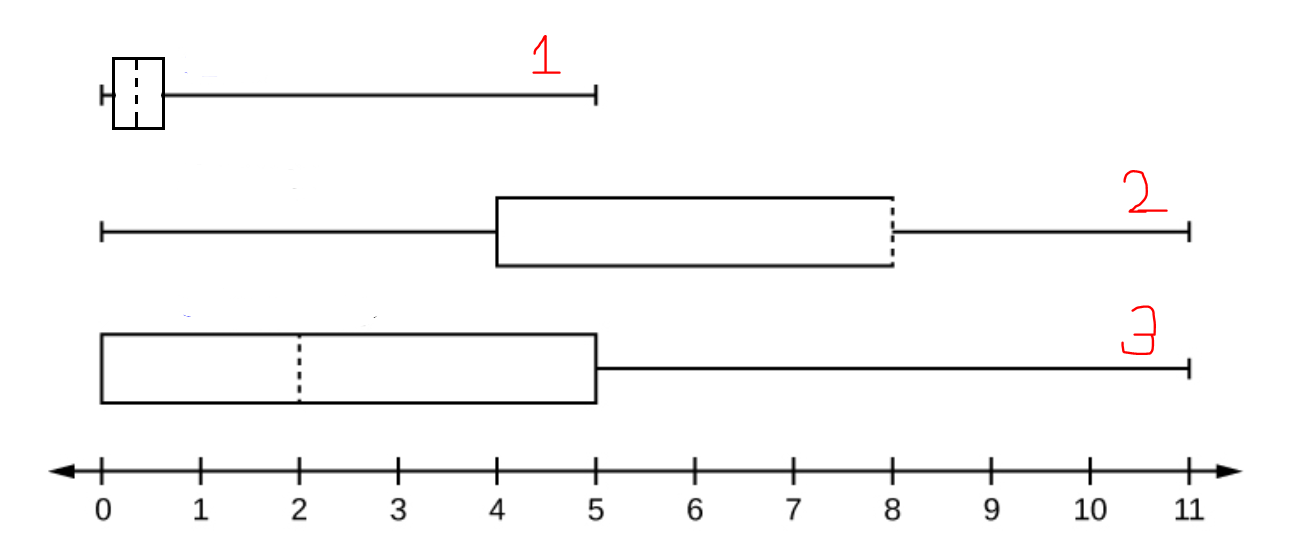
\includegraphics[width=0.7\textwidth]{boxplot_qna.PNG}
        \caption{\label{fig:1} Box plot for Q1.}
    \end{figure}
    % \item 
    \item After spinning a random real number generator $n$ times which generates a number between $0-10$, we get that the mean is around $5.4$, and the median is $5.5$. Moreover, only 7 \% of the total samples are above $8.4$, and only 6.8 \% of the samples are less than $2.4$. The standard deviation of values is around $1.5$. What can you say about the skew of this distribution? What about the kurtosis?   
    % \item Note that the median number of paperbacks read is less than the median number of ebooks read, but the mean number of paperbacks and eboosks read is quite close. How is this possible? 
    % \item
\end{enumerate}

Answer:
\newline Part (a): Let the frequency of occurence of $i$ books read be $x_i$ for $i=0,1,..4$. Note that we have 5 variables, and we can construct 5 equations- one for total number of people, and the rest corresponding to each reported descriptive value. We can represent it as a system in 5 variables as follows using the corresponding expressions for sample mean, sample variance (i.e. s), skew and kurtosis.
\[ 
\implies 
\begin{bmatrix}
1 & 1 & 1 & 1 & 1 \\
0 & 1 & 2 & 3 & 4 \\
\mu^2 & (1-\mu)^2 & (2-\mu)^2 & (3-\mu)^2 & (4-\mu)^2 \\
-\mu^3 & (1-\mu)^3 & (2-\mu)^3 & (3-\mu)^3 & (4-\mu)^3 \\
\mu^4 & (1-\mu)^4 & (2-\mu)^4 & (3-\mu)^4 & (4-\mu)^4 \\
\end{bmatrix}
\begin{bmatrix}
x_0 \\
x_1 \\
x_2 \\
x_3 \\
x_4 \\
\end{bmatrix}
= \begin{bmatrix}
n \\
n\mu \\
(n-1)s^2 \\
ns^3 \eta \\
ns^4*(\gamma+3)
\end{bmatrix}
\]
Applying row transformations on the linear system- $R3 \to R3 - \mu^2 R1 + 2\mu R2$-
\[
\begin{bmatrix}
1 & 1 & 1 & 1 & 1 \\
0 & 1 & 2 & 3 & 4 \\
0 & 1 & 2^2 & 3^2 & 4^2 \\
% 0 & 1 - 2\mu & (2-\mu)^2 & (3-\mu)^2 & (4-\mu)^2 \\
-\mu^3 & (1-\mu)^3 & (2-\mu)^3 & (3-\mu)^3 & (4-\mu)^3 \\
\mu^4 & (1-\mu)^4 & (2-\mu)^4 & (3-\mu)^4 & (4-\mu)^4 \\
\end{bmatrix}
\begin{bmatrix}
x_0 \\
x_1 \\
x_2 \\
x_3 \\
x_4 \\
\end{bmatrix}
= \begin{bmatrix}
n \\
n\mu \\
(n-1)s^2 + \mu^2n \\
ns^3 \eta \\
ns^4*(\gamma+3)
\end{bmatrix}
\]
Applying row transformations on the linear system- $R4 \to R4 + \mu^3 R1 - 3\mu^2 R2 + 3\mu R3$-
\[
\begin{bmatrix}
1 & 1 & 1 & 1 & 1 \\
0 & 1 & 2 & 3 & 4 \\
0 & 1 & 2^2 & 3^2 & 4^2 \\
% 0 & 1 - 2\mu & (2-\mu)^2 & (3-\mu)^2 & (4-\mu)^2 \\
0 & 1^3 & 2^3 & 3^3 & 4^3 \\
\mu^4 & (1-\mu)^4 & (2-\mu)^4 & (3-\mu)^4 & (4-\mu)^4 \\
\end{bmatrix}
\begin{bmatrix}
x_0 \\
x_1 \\
x_2 \\
x_3 \\
x_4 \\
\end{bmatrix}
= \begin{bmatrix}
n \\
n\mu \\
(n-1)s^2 + \mu^2n \\
ns^3\eta + \mu^3 n + 3(n-1)s^2\mu \eta \\
ns^4*(\gamma+3)
\end{bmatrix}
\]

Applying row transformations on the linear system- $R5 \to R5 - \mu^4 R1 + 4\mu^3 R2 - 6\mu^2 R3 + 4 \mu R4$-
\[
\begin{bmatrix}
1 & 1 & 1 & 1 & 1 \\
0 & 1 & 2 & 3 & 4 \\
0 & 1 & 2^2 & 3^2 & 4^2 \\
% 0 & 1 - 2\mu & (2-\mu)^2 & (3-\mu)^2 & (4-\mu)^2 \\
0 & 1^3 & 2^3 & 3^3 & 4^3 \\
0 & 1^4 & 2^4 & 3^4 & 4^4 \\
\end{bmatrix}
\begin{bmatrix}
x_0 \\
x_1 \\
x_2 \\
x_3 \\
x_4 \\
\end{bmatrix}
= \begin{bmatrix}
n \\
n\mu \\
(n-1)s^2 + \mu^2n \\
ns^3\eta + \mu^3 n + 3(n-1)s^2\mu \\
ns^4*(\gamma+3) -2\mu^2(n-1)s^2 - 2\mu^4 n + 4\mu n s^3 \eta  
\end{bmatrix}
\]
Since we arrive at an invertible matrix on the LHS, the solution of the linear homogeneous system exists. Hence, Jane can substitute the values that she has and calculate respective frequency values. She just needs to make sure that the solution is also integral - if the solution isn't integral for the given values then, there must be some error in the calculated descriptive values. The best way to visualize this frequency table is using a bar chart.
\newline Part (b): Box plot 1 is extremely skewed to the right, 75\% of the values fall below 2 months. For box plot 2, the lower 50 \% is more spread out than the upper half, so it is skewed to the left. At least 50 \% of sales represented by box plot 2 are after 8 months. The third box plot is also skewed to the right, most of the sales in box plot 2 took place in the first half of 2020. We deduce that 1 represents offline sales of paperbacks (since 2020 had the pandemic going on, which restricted free offline movement). We deduce that 2 represents sales of paperbacks online (again, due to the pandemic and shutting down of online delivery options, it is presumable that most sales would've taken place after a considerable relaxation in lockdown). Thus, we deduce that 3 represents sales of e-books online- since the availability of paperbacks was heavily impacted in the first half of the year everyone who wanted to read must've downloaded e-books instead. 
\newline Part (c): We can't comment on the skew without more information about the mode since the median and mean are very close. 
\newline For the kurtosis, we proceed by comparing this to a standard normal distribution. Note that the median is slightly larger than the mean, and the right tail seems to have more data than the left. Comparing this to a normal distribution with mean 5 and standard deviation $1.5$ we would get that 95 \% of the samples lie within $[5.4-2*1.5,5.4+2*1.5] = [2.4,8.4]$ which implies only $~2.5 \%$ of the total samples would lie beyond 8.4 or less than 2.4 for a normal distribution. That is not the case here. Here the tails are 'heavier' than a normal distribution, thus it is Leptokurtic. 

\item	Descriptive Statistics
\begin{enumerate}
    % \item IPL correlation between earning and runrate  
    \item If a runner is in the 95th percentile of a marathon race, with a time of around 1 hours and 50 mins, are they amongst the fastest? Why or why not? How does this compare to the position of a student in the 95th percentile of JEE Mains? 
    \item Kevin is trying to compare the weather phenomena of Manali with California. Throughout 6 days, he notes down the reported temperatures at 7 P.M. IST as [5, 10, 0, 15, 20, 25] in Manali, and [41, 50, 32, 59, 69, 77] in California respectively. Next, he computes the coefficient of variation for Manali as 0.82 and California as 0.34 respectively - and concludes that one should live in California because the extent of variation of temperature is less. He has made a major mistake here! Correct him. [Hint- what are the standard units of temperature used in either country?]
    \item You have to invest in $10,00,000$ in plastic-based charger enclosures in the next $3$ years for your mobile charger development start-up, and you're extremely scared of losing this money. So you decide to hedge against the risk of a potential increase by buying contracts, such that each contract guarantees $40,000$ enclosures. If standard deviation of changes in cost of plastic-based enclosures in next $3$ years is $0.032,$ standard deviation of changes in per-enclosure cost is $0.040,$ and both are correlated by $0.8$ - how many contracts should you buy to minimize variance of your net cost?   
\end{enumerate}
Answer:
\newline Part (a): A runner in the 95th percentile is actually slower than 95 \% of the population (since they take more time), but a student at the 95th percentile of JEE Mains is ahead of 95 \% of the population (since their score is higher). 
\newline Part (b): Note the difference in values of the temperature ranges- this can help us conclude that Kevin has made a mistake by not noting down the corresponding units of temperatures! Since in India temperatures are reported in Celsius, and in the USA temperatures are reported in Fahrenheit- we conclude that Kevin has compared 2 relative scales, without bringing them down to the same unit. On converting both of these temperature data to the Kelvin scale, we get that the absolute temperatures are exactly the same! Thus, Kevin is wrong about California being the better place to live. 
\begin{table}[!ht]
\centering
\begin{tabular}{lllllll}
Manali     & 278.15 & 283.15 & 273.15 & 288.15 & 293.15 & 298.15 \\
California & 278.15 & 283.15 & 273.15 & 288.15 & 293.15 & 298.15
\end{tabular}
\end{table}
\newline Part (c): Let X represent buying in future, Y represent hedging. Let $C$ be no. of contracts, here we would like to minimize- 
$$Var(X,Y) =  (C.40,000)^2 \sigma_Y^2 + (10,00,000)^2\sigma_X^2- 2(-10,00,000)(40,000)(C)\sigma_X^2\sigma_Y^2\rho$$
Note that potential buying of 10,00,000 enclosures can be considered as holding -10,00,000 enclosures. 
Since it's a quadratic in $C,$ min value would be at 
$$C = \dfrac{-b}{2a} = \dfrac{\sigma_X \rho 10,00,000}{\sigma_Y 40,000} = 16$$.
Thus, one should buy 16 such contracts to minimize variance in expenditure. 
\item	Sampling Distributions
\begin{enumerate}
    \item For $X_1, X_2, . . . , X_n$ independent samples from an infinite population. Assume the distribution they're sampled from has some continuous pdf $f(x)$ and cdf $F(X)$, and find the density of the $k$'th order statistic in terms of these. 
    \item For the samples from part (a) - define $\bar{X_k}$ and $S_k^2$ as the sample mean and sample variance of first $k$ samples respectively. Define $S_{n-k}^2$ as $\dfrac{\Sigma_{i=k+1}^{n}(X_i-\dfrac{\Sigma_{i=k+1}^{n} X_i}{n-k})}{(n-k-1)}$. What is the sampling distribution of $\dfrac{S_k^2}{S_{n-k}^2}$? State any required assumption on the distribution of $X_i$'s.
    \item Consider all notation as defined in previous part. What is the distribution of
    \newline $\dfrac{(k-1)S_k^2 + (n-k-1)S_{n-k}^2}{\sigma^2}$? Express that in terms of i.i.d standard normal distributed variates, and prove that if these variates are subjected to $m$ independent and homogeneous linear constraints, then there's a reduction of $m$ in the degree of freedom of the original distribution. Consider a constraint of the form $AX=0,$ where $A$ is a full-rank matrix of dimensions $m \times n$ and the rows are unitary and mutually orthogonal.

\end{enumerate}
Answer:
\newline Part (a): 
Let $Y$ represent the $k$'th order statistic. Then, 
$$P(Y \le x) = \Sigma_{i=k}^{n} {n \choose i} P(X_i \le x)^{i}(1-F(x))^{n-i}$$
because for k'th order statistic to be less than $x$ we need at least $k$ or more samples to have observed value less than $x$ and rest should be more than $x$. Then we proceed case wise, and since each case is mutually exclusive we sum it up. 
To find the density function, we need to differentiate this with respect to x, since CDF of Y is $P(Y \le x)$. On differentiating, we get

$$f_Y(x) = \Sigma_{i=k}^{n} {n \choose i} [i*F(x)^{i-1}(1-F(x))^{n-i}f(x) - (n-i)*F(x)^{i}(1-F(x))^{n-i-1}f(x)]$$
$$ = [n*{n-1 \choose i-1}F(x)^{i-1}(1-F(x))^{n-i}f(x)] - [n*{n-1 \choose n-i-1}F(x)^{i}(1-F(x))^{n-i-1}f(x)]$$
$$ = \Sigma_{i=k}^{n} [n*{n-1 \choose i-1}F(x)^{i-1}(1-F(x))^{n-i}f(x)] - [n*{n-1 \choose i}F(x)^{i}(1-F(x))^{n-i-1}f(x)]$$
by using properties of $n \choose r$. Note that the terms will get cancelled (this is similar to a telescopic series sum) and only first term will remain. Therefore, 
$$f_Y(x) = n {n-1 \choose k-1} F(x)^{k-1} (1-F(x))^{n-k} f(x)$$. This is the sampling distribution of k'th order statistic. 

 Part (b): As defined, we would have $\bar{X_k} = \Sigma_{i=1}^{k} X_i$ and $(k-1)S_k^2 = \Sigma_{i=1}^{k} (X_i-\bar{X_k})^2$. 
Now, we know that by CLT, $\bar{X_k} \sim N(\mu,\frac{\sigma^2}{\sqrt{n}})$ as $k \to \infty$. But we can't make any conclusive remarks about $S_k,$ thus we proceed with the assumption that $X_i \sim N(\mu,\sigma^2)$. For such a case, we know that $\dfrac{(k-1)S_k^2}{\sigma^2} \sim \chi_{k-1}^2$. Therefore, $\dfrac{(k-1)S_k^2}{(n-k-1)S_{n-k}^2} \sim \dfrac{\chi_{k-1}^2}{\chi_{n-k-1}^2}$ since $S_k$ and $S_{n-k}$ are independent because $S_k$ is a function of $X_1,X_2,..X_k$ and $S_{n-k}$ is a function of $X_{k+1},..X_n$. 
So, 
$$\dfrac{S_k^2}{S_{n-k}^2} \sim \dfrac{(n-k-1)\chi_{k-1}^2}{(k-1)\chi_{n-k-1}^2} \implies \dfrac{S_k^2}{S_{n-k}^2} \sim F_{k-1,n-k-1}$$. 

Part (c): From part (b), we can say that
$$\dfrac{(k-1)S_k^2}{\sigma^2} + \dfrac{(n-k-1)S_{n-k}^2}{\sigma^2} \sim \chi_{k-1}^2 + \chi_{n-k-1}^2 \sim \chi_{n-k-1+k-1}^2 \sim \chi_{n-2}^2$$. Then, if we have iid $Z_1,Z_2,..Z_{n-2} \sim N(0,1),$ we would get $\Sigma_{i=1}^{n=2} Z_i^2 \sim \chi_{n-2}^2$. 
\newline Consider the constraint $AZ = 0,$ where $A$ is a full rank $m \times n-2$ matrix. Since the rows of A are mutually orthogonal and unitary, the set of all rows must form a linearly independent subset of $R^{n-2},$ thus it can be extended to an orthogonal basis of $R^{n-2}$- the way we proceed is we first pick a vector not in the span of the current set and keep adding it till we have $n-2$ elements in our set. Then we apply Gram-Schmidt process to make the rows mutually orthogonal. Now, construct a $B, n-2\times n-2$ matrix using this extended basis. Clearly, by definition of Gram Schmidt, the first m rows of $B$ are identical to $A$. 
We define $Y = BZ$, where $Y = (Y_1, Y_2, .., Y_{n-2})^T$ and $Z = (Z_1,Z_2,..,Z_{n-2})^T$. 
The density of $Y$ is $\dfrac{exp(\dfrac{-Y^TY}{\sigma^2})|J|}{(\sigma \sqrt{2\pi})^{n-2}}$ where $J$ is the jacobian (since $Y$ is a function of $X$), and $J = \dfrac{ \delta Z}{\delta Y} = \dfrac{1}{|A|} \implies |J| = 1$. Thus, $Y_i's$ are independent and standard normal distributed random variables (their joint distribution can easily be factorized). 

$$\implies \Sigma_{i=1}^{n-2} Z_i^2 = \Sigma_{i=1}^{n-2} Y_i^2 = \Sigma_{i=m+1}^{n-2} Y_i^2$$ because of the constraint that $AZ=0$. 
Thus, $\Sigma_{i=1}^{n-2} Z_i^2 \sim \chi_{n-2-m}^2$.
% \newline Part (c)

\item Sampling Distributions 
\begin{enumerate}
    \item In 2 independent experiments from the same infinite sized and normal distributed population, we sample $n+1$ points from experiment $A$ and $m+1$ points from experiment $B$. What is the probability that the observed sample variance of experiment $A$ is higher than that of experiment $B$ at least by a factor of $k > 0$?
    \item Consider $X = \Sigma_{i=1}^{k} \frac{(n_i - f_i)^2}{f_i}$, where $f_i$ is the expected frequency of class $i, n_i$ is the observed frequency, and $\Sigma_{i=1}^{k} n_i = N$. What is the distribution of $X$ as $\Sigma_{i=1}^{k} n_i \to \infty$ and $n_i$ are also sufficiently large? What does this reduce to for $k=3$?
    \item Given independent $X_i \sim N(g(i),(g(i))^2),$, where $g(i)$ is an invertible, real function of $i$, construct a statistic such that it has a student's T distribution with $n$ degrees of freedom. 
    % \item State the sampling distributions of $\dfrac{\Sigma_{i=1}^{n} (X_i-\mu)^2}{\sigma^2}$ and $\dfrac{\Sigma_{i=1}^{n} (X_i-\bar{X})^2}{\sigma^2}$. Are they different (yes/no)? If yes, why? Explain the difference qualitatively. 
\end{enumerate}
Answers:
\newline Part (a): Notice that $\dfrac{nS_A}{\sigma^2} \sim \chi_{n}^2$ and $\dfrac{mS_B}{\sigma^2} \sim \chi_{m}^2$, so, $\dfrac{S_A}{S_B} \sim F_{n,m}$, where $S_A,S_B$ are sample variance of experiments A and B respectively. Thus, for $S_A \ge k*S_B,$ we need to find $P(\dfrac{S_A}{S_B}\ge k) = P(F_{n,m} \ge k) = 1 - P(F_{n,m} \le k) = 1 - F_{n,m}(k),$ where $F_{n,m}$ represents CDF of F distribution. 
\newline Part (b): Let $p_i$ be the probability of sampling from class $i$, then 
$$P(n_i \text{ in 'th class} \forall i) = P = \dfrac{n! \Pi_{i=1}^{k} p_i^{n_i}}{n_1!...n_i!--n_k!}$$ where $n = \Sigma_{i=1}^{k} n_i$.
Now, take $lim_{n \to infty} P$, and use Stirling's approximation for the asymptotic value of $n!$, i.e. $n! \sim \sqrt{2\pi n} (\dfrac{n}{e})^n$, we get

$$P \sim \dfrac{n^n\sqrt{n}}{\sqrt{2\pi}^{k-1} \Pi_{i=1}^{k} \sqrt{pi}} \times \Pi_{i=1}^{k} (\dfrac{p_i}{n_i})^{n_i+0.5} 
$$

$$\implies \sim \dfrac{1}{\sqrt{2\pi n}^{k-1} \Pi_{i=1}^{k} \sqrt{pi}} \times \Pi_{i=1}^{k} (\dfrac{n p_i}{n_i})^{n_i+0.5} 
$$
Now let $Q$ be $\dfrac{1}{\sqrt{2\pi n}^{k-1} \Pi_{i=1}^{k} \sqrt{pi}}$.
$$\implies log(P) \sim log(Q) + \Sigma_{i=1}^{k} (n_i + 0.5)\dfrac{np_i}{n_i} $$
$$\implies log(\dfrac{P}{Q}) \sim \Sigma_{i=1}^{k} (n_i + 0.5)\dfrac{f_i}{n_i}$$. 
Now, let $\eta_i$ be such that $\eta_i \sqrt{f_i} = n_i - f_i$. We'll show that they're asymptotically distributed as i.i.d standard normal random variables. 
Thus, we can write 
$$log(\dfrac{P}{Q}) \sim \Sigma_{i=1}^{k} -0.5 \eta_i^2 - \eta_i \sqrt{f_i}$$ after applying binomial theorem and neglecting higher powers of $f_i$ since we're taking the asymptotic case. Note that $\Sigma_{i=1}^{k} \eta_i \sqrt{f_i} = \Sigma_{i=1}^{k} n_i - f_i = n - n = 0$
$$log(\dfrac{P}{Q}) \sim \Sigma_{i=1}^{k} -0.5 \eta_i^2 \implies P \sim Q Exp(-0.5 \Sigma_{i=1}^{k} \eta_i^2)$$
So, $\eta_i \sim N(0,1)$, thus, 
$$\Sigma_{i=1}^{k} \dfrac{n_i-f_i}{f_i} \sim \Sigma_{i=1}^{k} \eta_i \sim \chi_{k-1}^2$$. $k-1$ because we've proved in Q3 that the existence of $m$ linear constraints means the degree of freedom decreases by $m,$ and here we have existence of one linear constraint i.e. $\Sigma_{i=1}^{k} (n_i - f_i) = 0$. 
\newline Part (c): We know that if we have $Z \sim N(0,1)$ and $Y \sim \chi_{n}^2$ then $\dfrac{Z}{\sqrt{Y/n}} \sim T_n$, so using this-
First define $Y_i = \dfrac{X_i - g(i)}{g(i)^2}$ and note $Y_i \sim N(0,1)$ so, 
$$\Sigma_{i=1}^{n} Y_i \sim \chi_{n}^2$$
Thus, $$\dfrac{Y_{n+1}\sqrt{n}}{\sqrt{\Sigma_{i=1}^{n} Y_i}} \sim T_n$$

\item	Point and Interval Estimations
\begin{enumerate}
    \item True or False: if $T_n(X_1,X_2,...X_n)$ is a consistent estimator for some $\theta$, then it is unique. 
    \item Given a continuous function $\psi,$ show that if $T_n(X_1,X_2,...X_n)$ is a consistent estimator for some $\theta$ then $\psi(T_n(X_1,X_2,...X_n))$ is a consistent estimator for some $(\psi(\theta))$.
    \item Steve Jobs has a population of $N$ red and green apple at Apple HQ. He samples $n$ apples with replacement and passes on this $n$ length binary string to Steve Wozniak- who is tasked with finding a consistent estimator of $p(1-p),$ where $p < 0.5$ is the probability of picking a green apple. You're the intern asked to help him with this- how will you go about it? Check if your resulting estimate is biased or not, if it is- state the value of the bias too.
    \item What's the value of lower bound of Cramer-Rao inequality for $\psi(p) = p(1-p)?$
    \item Find the method of moments estimate and maximum likelihood estimate for $p(1-p)$. Are they biased? 
    \item Another intern tells you that a non-zero bias implies that the apple supplier of Apple is "biased" towards red apples- how will you correct him?  

\end{enumerate}

Answer: 
\newline Part (a): False. Given a consistent $T_n$, consider the statistic $\dfrac{n+1}{n-1} T_n$. Note that as $n \to \infty,$ 
$$\dfrac{n+1}{n-1} T_n \to T_n, T_n \to \theta \implies \dfrac{n+1}{n-1} T_n \to \theta$$
So, we have a counterexample. Thus $T_n$ is not unique. In fact we can construct a family of consistent estimators using this idea.
\newline Part (b): We're given that $T_n \to \theta$ in probability, and we need to show that $\psi(T_n) \to \psi(\theta)$. Since $\psi$ is continuous, by definition given an $\epsilon$ there exists $\delta$ s.t. 
$$|T_n - \theta| \le \delta \implies |\psi(T_n)-\psi(\theta)| \le \epsilon$$
Thus, the probability of $|\psi(T_n)-\psi(\theta)| \le \epsilon$ is at least the probability of occurrence of $|T_n - \theta| \le \delta$ so, 
$$P(|\psi(T_n)-\psi(\theta)| \le \epsilon) \ge P(|T_n - \theta| \le \delta) \implies  0 \le P(|\psi(T_n)-\psi(\theta)| > \epsilon) \le P(|T_n - \theta| > \delta)$$
Thus, by sandwich theorem we have that $\psi(T_n)$ is a sufficient estimator for $\psi(\theta)$.
\newline Part (c): Note that here we have $X_1,X_2,..,X_n$ samples such that $X_i \sim \Bernoulli(p)$. For Bernoulli distribution, we know that $\bar{X}$ is a consistent estimator of $p$. Note that $f(x) = x(1-x)$ is a polynomial, thus it must be continuous. So, from part (b) we can say that $f(\bar{X}) = \bar{X} (1-\bar{X})$ is a consistent estimator for $p(1-p)$.
\newline Finding bias of this estimator- note that $Y = \Sigma_{i=1}^{n} X_i \sim B(n,p)$, so
$$E(f(\bar{X})) = E(Y/n) - E(Y^2/n^2) = (1-\dfrac{1}{n})p(1-p) \neq p(1-p),$$ thus it is biased and the value of bias is $$bias = E(f(\bar{X})) - p(1-p) = -\dfrac{1}{n}p(1-p)$$. 
\newline Part (d): Here, $I(\theta) = -E(\dfrac{\delta^2 log(f_{\theta}(x))}{\delta^2 \theta})$ so, since $f_{p} (x) = \Pi_{i=1}^{n} p^{X_i} (1-p)^{1-X_i}$
$$ I(p) = \dfrac{E(\Sigma_{i=1}^{n} X_i)}{p^2} + \dfrac{E(\Sigma_{i=1}^{n} (1-X_i))}{(1-p)^2} = \dfrac{n}{p(1-p)} 
$$
and $\psi'(p) = 1-2p$ so lower bound is $$
\dfrac{(\psi'(p))^2}{I(p)} = \dfrac{(1-2p)^2p(1-p)}{n}
$$
Part (e): Note that method of moments estimate is same as the consistent estimate found in part (c) because by method of moments we'll get $p = \bar{X}$ since Bernoulli depends only on one parameter $p$.
To find MLE for $p(1-p),$ first we write the log likelihood function as 
$$log(L) = \Sigma_{i=1}^{n} (X_i log(p) + (1-X_i) log(1-p))$$
Now we need to differentiate it wrt $\theta = p(1-p),$ so we do-
$$\dfrac{\delta log L}{\delta \theta} = \dfrac{\delta log L}{\delta p}*\dfrac{\delta p}{\delta \theta} = 0 \iff \dfrac{\delta log L}{\delta p} = 0$$ because
$$ p(1-p) = \theta \implies (1-2p)\dfrac{\delta p}{\delta \theta} = 1 \implies \dfrac{\delta p}{\delta \theta} \neq 0, \forall p <0.5$$
But this is similar to expression for MLE of $p$ which is also $\bar{X}$ thus, in this case we get MLE of $p(1-p)$ is also $\bar{X} (1-\bar{X})$ and same as the estimator we get from method of moments. 
Part (f): There is a HUGE difference between both biases! You must tell him that the probability of the "biased" choice of a red apple depends on the parameter $p$, and since it's given that $p<0.5$ it means that the probability of picking a red apple is $1-p > 0.5$, in this sense the sampling is biased - because probabilities of picking a red apple is larger than that of picking a green. The bias being talked about here is that of an estimator- which is the difference between the expected value of estimator and the true value of the parameter that we're trying to estimate. 

\item	Point and Interval Estimations
\begin{enumerate}
    \item We have 4 normal distributions of same variance $\sigma^2$ and we sample 4 different sets of size $n$ from each independently. It is known that the population means are $\mu_1 + \mu_2 + \mu_3$, $\mu_1 - \mu_2 - \mu_3$, $\mu_1 + \mu_2 - \mu_3$, $\mu_1 - \mu_2 + \mu_3$ for each of the 4 distributions. Consider $\sigma^2$ to be known, what's the MLE for $\mu_1,\mu_2,$ and $\mu_3$?

   \item Let $X_1, X_2,..X_n$ be iid observations from a distribution with density
    $f_{\alpha}(x) = \dfrac{\alpha}{(x+1)^{1+\alpha}},$ for $x, \alpha \in (0,\infty)$. Find a sufficient statistic for this.
    \item In a random sample of 800 voters before 2016 US Presidential elections, 144 preferred Trump over Obama. What's the 90\% confidence interval for the overall proportion of voters who prefer Obama over Trump?

\end{enumerate}
Answers:
\newline Part (a): Note that the 4 samples are independent. For the i'th distribution, we consider a sequence $X_{i1},X_{i2}...X_{in} \sim N(mean_i, \sigma^2)$. The log likelihood function can be written as

$$
log L = log (\dfrac{1}{\sigma\sqrt{2\pi}})^{4n}) \times Exp [
\dfrac{-1}{2\sigma^2} ( \Sigma_{i=1}^{4} \Sigma_{j=1}^{4} (X_{ij} - mean_i)^2)])
$$
$$\implies log L = -4n log(\sigma^2) - \dfrac{1}{2\sigma^2}
[\Sigma_{i=1}^{4} \Sigma_{j=1}^{4} (X_{ij} - mean_i)^2]
$$
To find MLE of $\mu_1,\mu_2,\mu_3$ we need to solve $\dfrac{\delta logL}{\delta \mu_i} = 0, i = 1,2,3$
Now, 
$$\dfrac{\delta logL}{\delta \mu_1} = 0$$ 
$$\implies \Sigma_{i=1}^{4} \Sigma_{j=1}^{n} (X_{ij}) + n[(-\mu_1+\mu_2+\mu_3)+(-\mu_1-\mu_2+\mu_3)+(-\mu_1+\mu_2-\mu_3)+(-\mu_1-\mu_2-\mu_3)] = 0$$
$$\implies \mu_1 = \dfrac{\bar{X_1}+\bar{X_2}+\bar{X_3}+\bar{X_4}}{4}$$
Similarly,
$$\dfrac{\delta logL}{\delta \mu_2} = 0$$ 
$$\Sigma_{j=1}^{n} (X_{1j} + X_{2j} - X_{3j} - X_{4j}) + n[(-\mu_1+\mu_2+\mu_3)-(-\mu_1-\mu_2+\mu_3)+(-\mu_1+\mu_2-\mu_3)-(-\mu_1-\mu_2-\mu_3)] = 0$$
$$\implies \mu_2 = \dfrac{\bar{X_1}+\bar{X_2}-\bar{X_3}-\bar{X_4}}{4} 
$$
And,
$$\dfrac{\delta logL}{\delta \mu_3} = 0$$ 
$$\Sigma_{j=1}^{n} (X_{1j} - X_{2j} + X_{3j} - X_{4j}) + n[(-\mu_1+\mu_2+\mu_3)+(-\mu_1-\mu_2+\mu_3)-(-\mu_1+\mu_2-\mu_3)-(-\mu_1-\mu_2-\mu_3)] = 0$$
$$\implies \mu_3 = \dfrac{\bar{X_1}-\bar{X_2}+\bar{X_3}-\bar{X_4}}{4} 
$$
where $n \bar{X_i} = \Sigma_{j=1}^{n} X_{ij}, i=1,2,3,4$.

Part (b): For a i.i.d sample of size $n$, we have 
$$f_{\alpha}(X) = \Pi_{i=1}^{n} \dfrac{\alpha}{(1+X_i)^{1+\alpha}} = \dfrac{\alpha^n}{\Pi_{i=1}^{n}(1+X_i)^{1+\alpha}}$$
Now, consider $T_n = \Pi_{i=1}^{n} (1 + X_i),$ then,
$$f_{\alpha}(X) = \dfrac{\alpha^n}{T_n^{1+\alpha}}$$
Thus, $T_n$ is a sufficient statistic by applying factorization theorem, where $g(T_n, \alpha) = f_{\alpha}(X)$ and $h(X) = 1$. 
\newline Part (c): $n=800, O = \dfrac{800-144}{800}$ is the proportion of voters who prefer Obama. 
$0.5\alpha = \frac{5}{100}$, so $t_{n,0.5\alpha}= 1.645$ and confidence interval is $O \pm 1.645 \sqrt{\dfrac{O(1-O)}{n}}$, or confidence interval is $(0.818,0.822)$.
\end{enumerate} 

\end{document}
